\newpage

\section{Jak to wygląda w praktyce?}

\subsection{Podejście obiektowe}

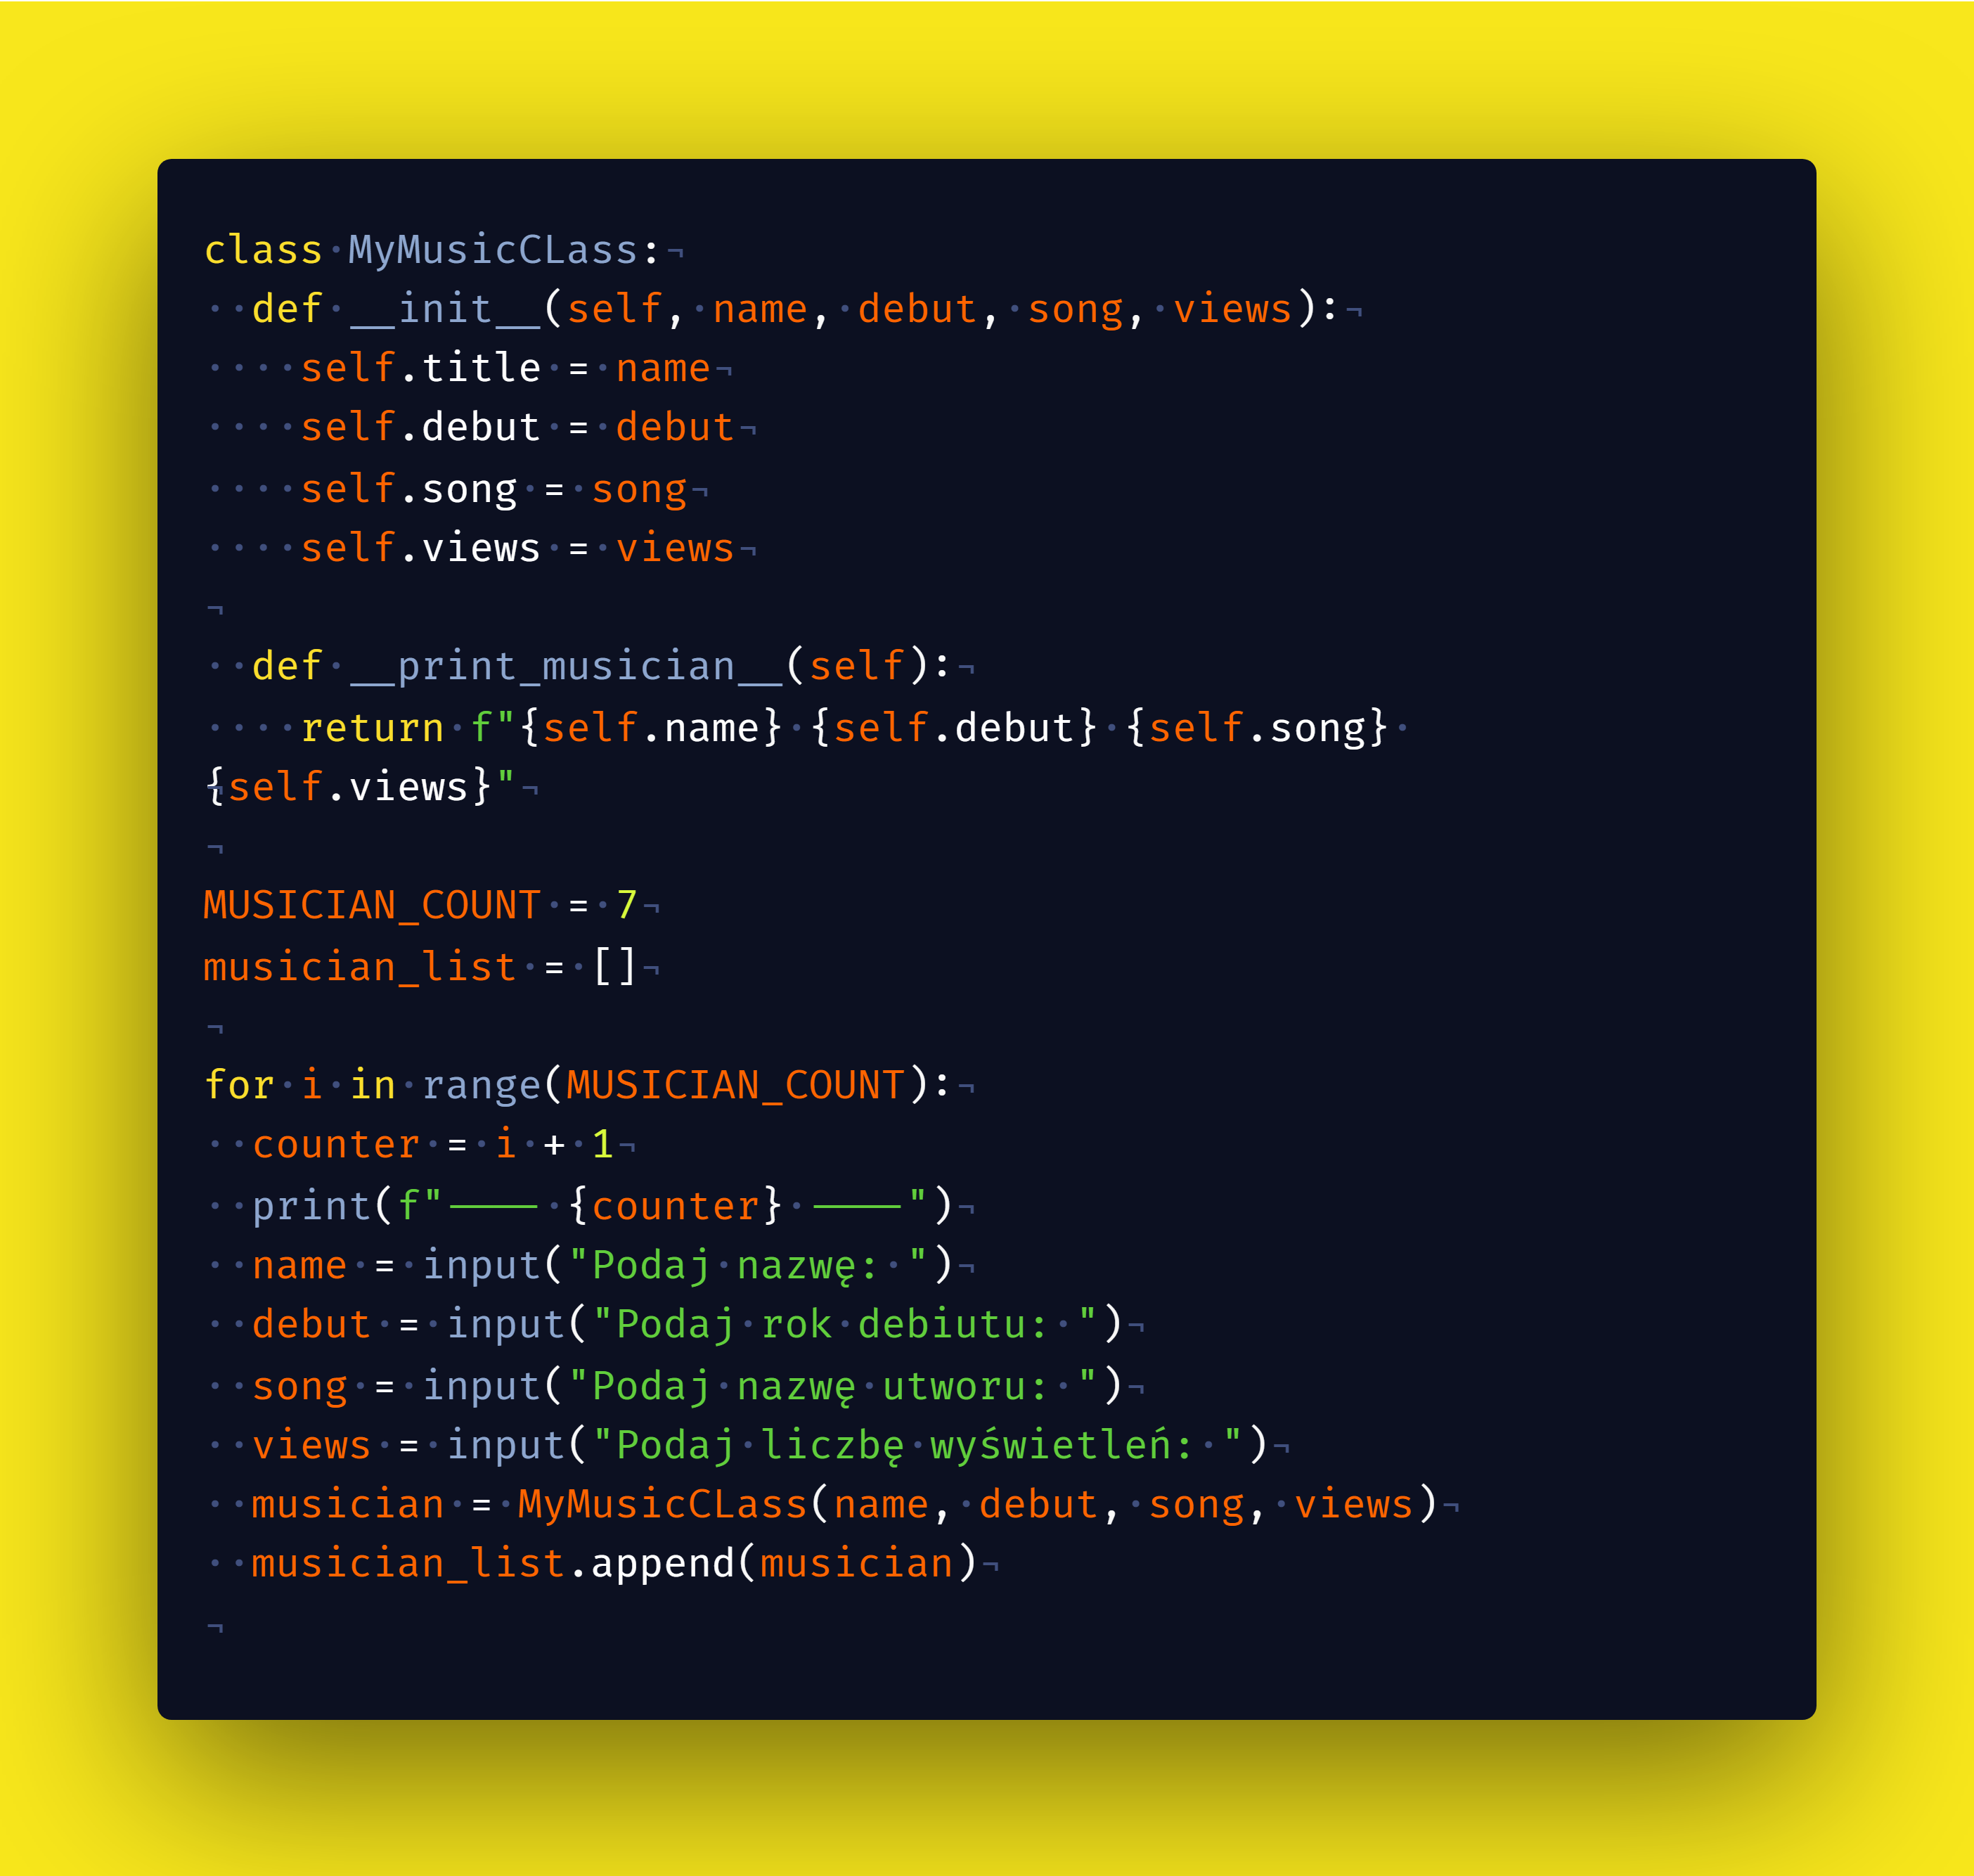
\includegraphics[width=\textwidth]{images/object-oriented-python.png}

\begin{flushleft}
    W tym przykładowym, i dość krótkim programie, możemy zauważyć jak dużo dodatkowych linii kodu należy napisać, aby uruchomić program obiektowy. Tworząc klasę dla poszczególnych twórców i twórczyń muzyki możemy w łatwy sposób stworzyć model dla ich późniejszego dodawania.
\end{flushleft} 

\begin{flushleft}
    Kod jest również dość przejrzysty i łatwo go edytować. Łącząc to podejście z czytelnością języka Python podejście obiektowe wydaje się bardzo dobre.
\end{flushleft}

\subsection{Program napisany proceduralnie}

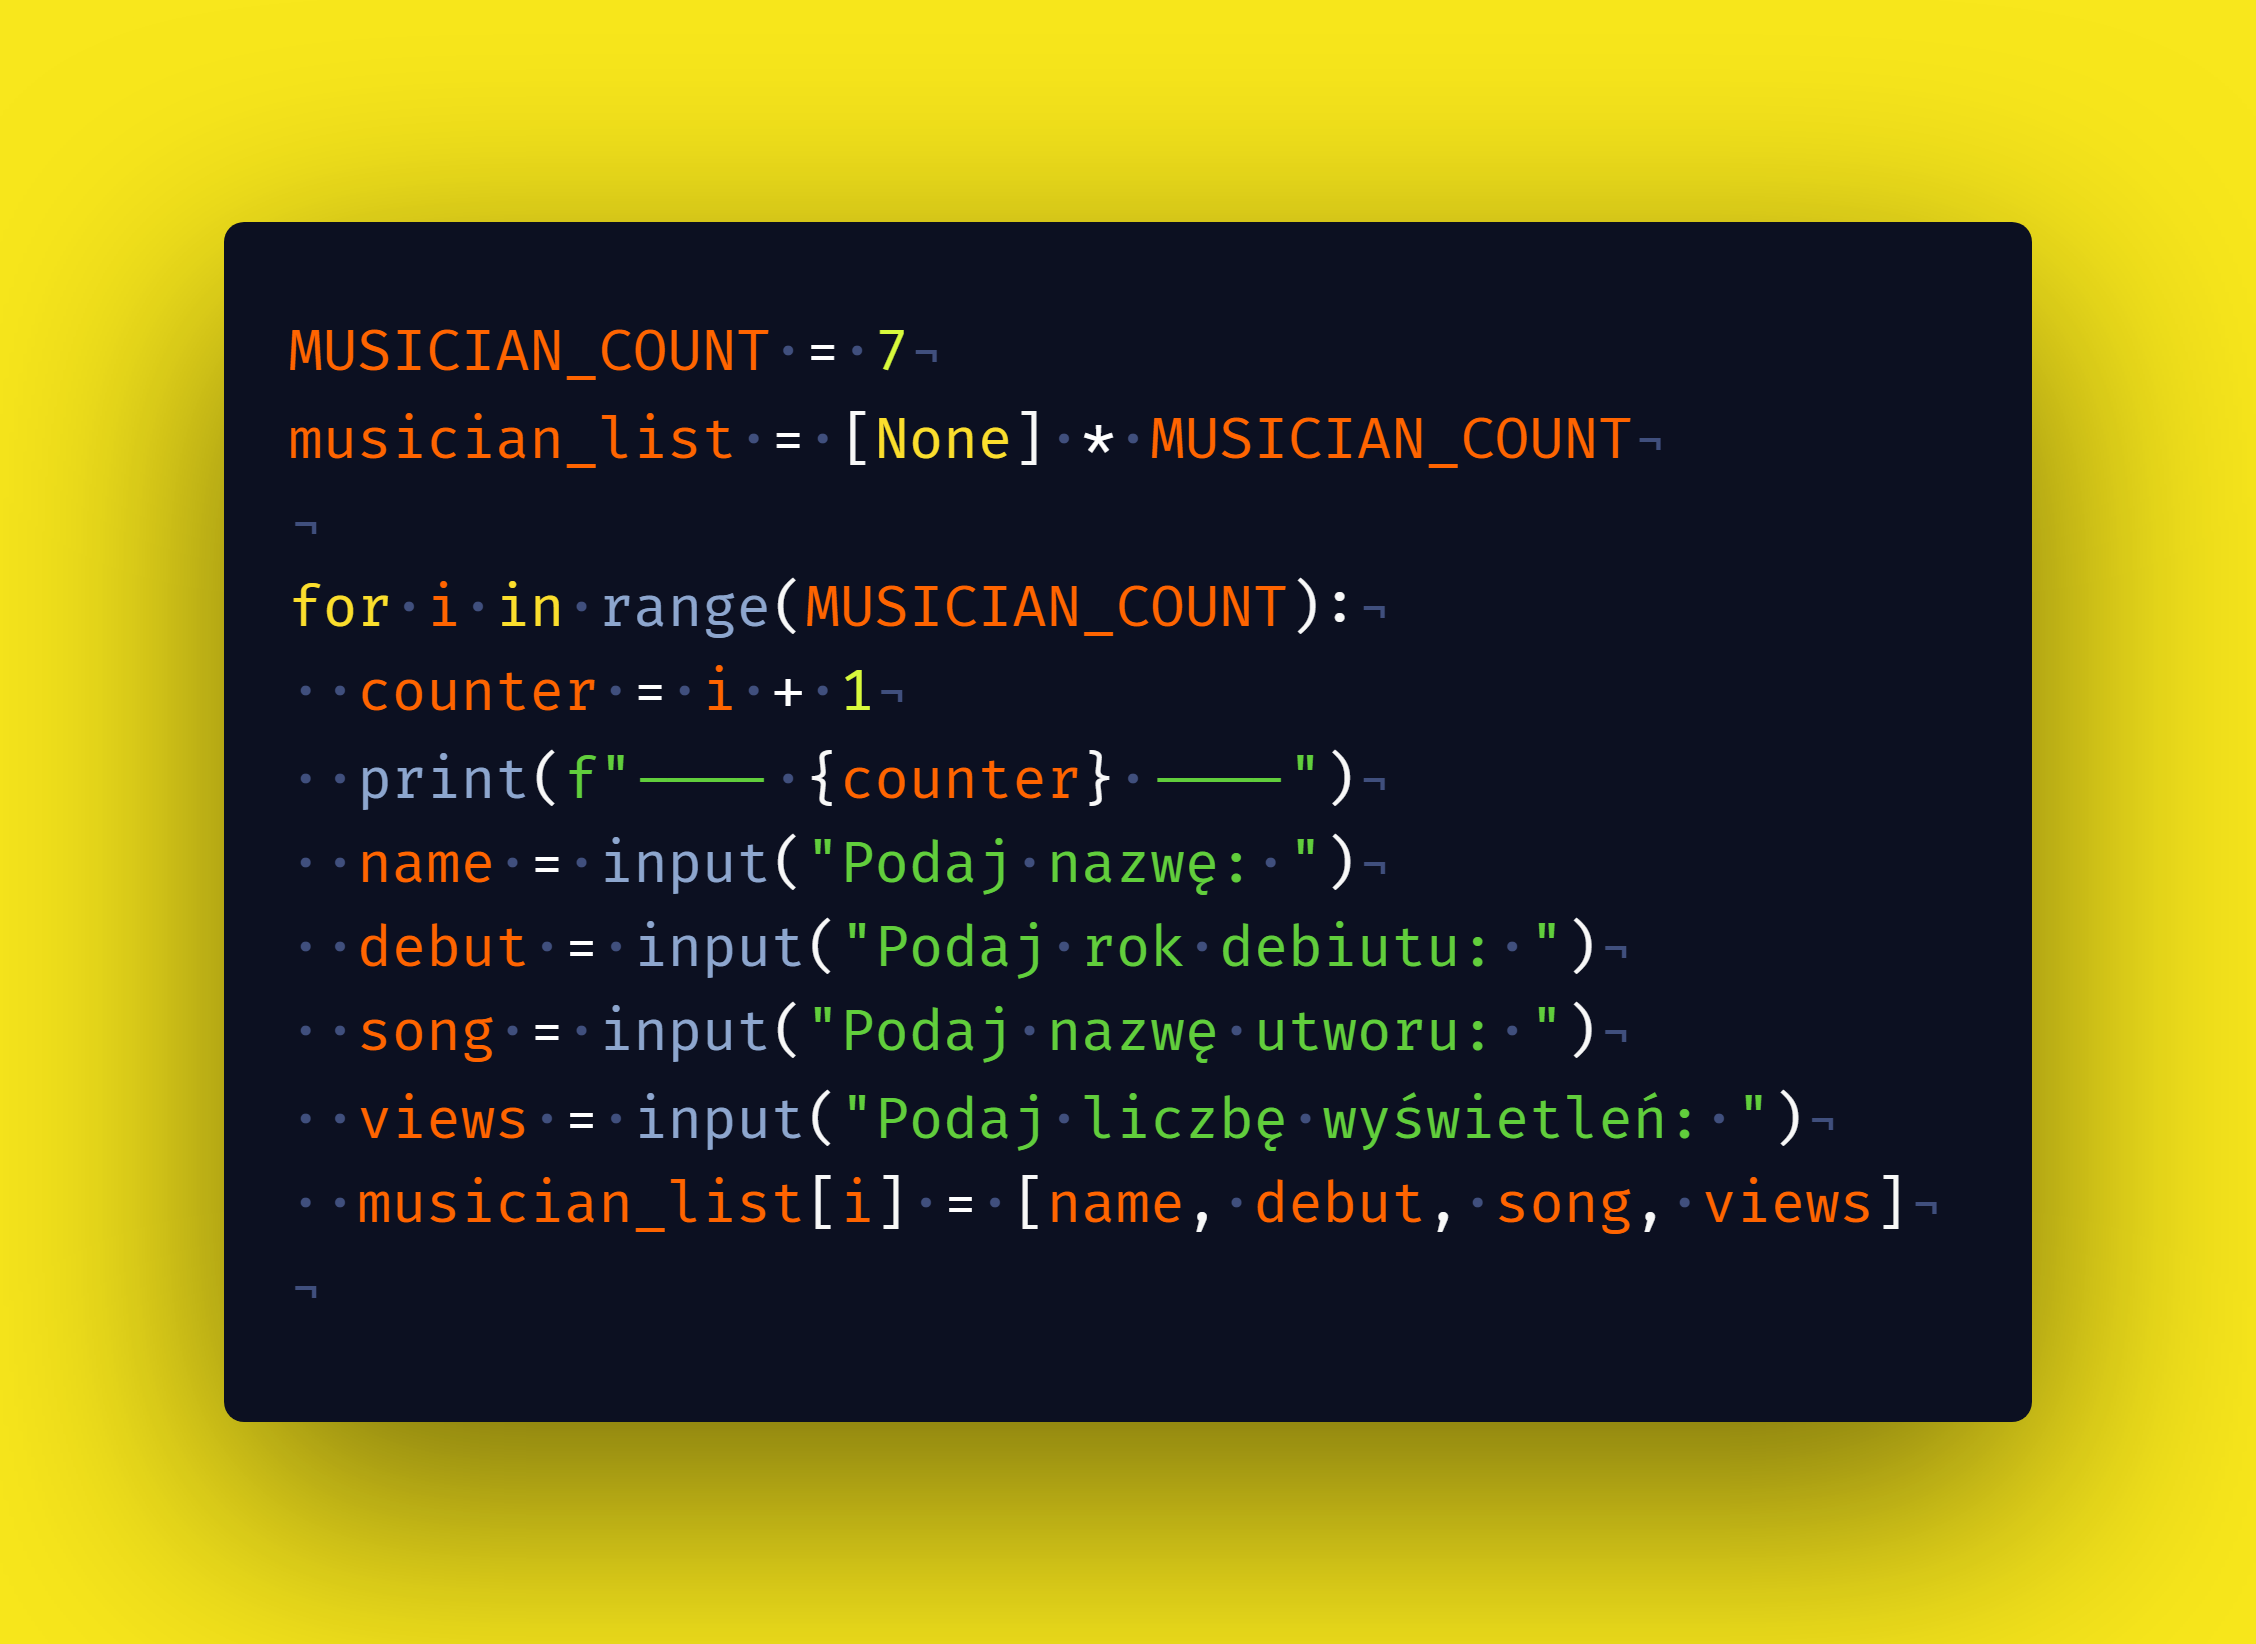
\includegraphics[width=\textwidth]{images/procedural-python.png}

\begin{flushleft}
    Kolejny przykład ilustruje program proceduralny. Jest krótszy i prostszy, ale ma jedną zdecydowaną wadę, aby wykonać zadanie - dać możliwość dodawania swojej ulubionej muzyki, należało zastosować trik. 
\end{flushleft}

\begin{flushleft}
    Zamiast tworzyć poszczególne obiekty wszystkie dane zapisujemy w \emph{tablicy dwuwymiarowej}. Każdy \emph{indeks} pierwszego wiersza będzie definiować jeden rekord w bazie, co może sprawiać kłopoty w odczytywaniu struktury zapisu danych.
\end{flushleft}
